\section{Introduction}\label{sec:introduction}
\mycite{Fanger1970} developed the \ac{pmv} model, which is now incorporated into the \gls{7730} standard~\cite{iso7730} in its original form.
The \ac{pmv} is an index that aims to predict the mean value of the thermal sensation votes (self-reported perceptions) of a large group of people on a sensation scale expressed from \num{-3} to \num{3} corresponding to the categories `cold,' `cool,' `slightly cool,' `neutral,' `slightly warm,' `warm,' and `hot.'~\cite{iso7730, ashrae552023}.
The \ac{pmv} model has been widely used worldwide by researchers and practitioners.
It is the most extensively used thermal comfort index.
A search within the article title, abstract, and keyword on Scopus with the search term `predicted mean vote' returns approximately \num{2050} documents.
Out of those \num{1200} are scientific peer-reviewed articles published in the research area of engineering, environmental science, social sciences, and energy.
This highlights this model's extensive adoption and use among the scientific community.
To this date, the \ac{pmv} remains to be the most utilized thermal comfort model even though several studies have highlighted that the \ac{pmv} has low accuracy in predicting thermal sensation votes~\cite{Cheung2019, Yao2022, Humphreys2002, doherty_evaluation_1988}.

\todo[inline]{Ed's comment:
The PMV model consists of a heat balance model and an empirical equation that predicts thermal sensation (PMV) from heat balance.  (need to describe this further, especially the simplified way that sweating is treated by the heat balance model).
In 2010 ASHRAE Std 55 modified the PMV heat balance calculation to make it more capable of predicting the cooling caused by elevated air movement under warm conditions.
It uses the Gagge two-node model to compute the convective and evaporative heat loss from the body. This model explicitly models physiological cooling in warm conditions where evaporation of sweat becomes a significant source of heat loss. The model output can be expressed as Standard Effective Temperature (SET) (provide citations to Gagge/Foblets). SET is implemented in Std 55 as an index to quantify the equivalent temperature reduction caused by air movement cooling. The reduced temperature is entered into the PMV heat balance model in a still air condition, from which the PMV index is calculated. This approach is intended to minimize errors introduced by the Fanger heat balance model’s reduced evaporative capacity on the predicted PMV result.
}
\todo[inline, color=blue!40]{
    FT similar to my previous comment. Firstly, I would like to mention here that the PMV does not at all try to estimate sweating. This is a problem, but neither the PMV nor the PMV CE do that.
    The Std 55 did not modify the PMV heat balance equation, instead it simply and only reduced the air and mean radiant temperatures by the cooling effect, this is not equivalent to doing an accurate heat balance calculation.
    The PMV CE consequently does not: 1) uses the Gagge two-node model to compute the convective and evaporative heat loss from the body 2) model explicitly models physiological cooling in warm conditions where evaporation of sweat becomes a significant source of heat loss.
    In addition, another comment about the PMV CE is that the cooling effect is not only applied in warm conditions but in fact it is applied in any conditions.
    SET is also a rather confusing variable since it is calculated not for a reference environment with standardised clo and met. But rather it is the temperature of a hypothetical isothermal environment at 50\% rh, <0.1 m/s (20 fpm) average air speed Va, and in which the total heat loss from the skin of an imaginary occupant wearing clothing, standardized for the activity concerned, is the same as that from a person in the actual environment with actual clothing and activity level.
    Finally, as you mentioned, \textit{The reduced temperature is entered into the PMV heat balance model in a still air condition, from which the PMV index is calculated.} this however do not ensure that the person is not feeling hot in this condition or sweating, consequently does not solve the issues that the original PMV has.
}

\subsection{\ac{pmv-ce} model}\label{subsec:pmv-ce-limitations}
The \gls{55} standard uses a modified version of the original model, the \ac{pmv-ce}~\cite{ashrae552023}.
The best source to see how \ac{pmv-ce} works is the standard itself, but the standard does not explain why some changes to the \ac{pmv} inputs were implemented, nor for example, why the \ac{ce} is subtracted from the \ac{tdb} and \ac{tr}.
A partial justification of the model is mainly described in \mycite{arens_moving_2009} and secondarily in \mycite{yang_cooling_2015}.
However, we could not find a peer-reviewed scientific publication that quantified the accuracy improvements of the model as implemented in the \gls{55} over the original \ac{pmv} model.

Figure~\ref{fig:flowchart_pmv_calculation} shows side by side the calculation routines for the \ac{pmv} and \ac{pmv-ce} models.
\begin{figure}[!htb]
    \begin{subfigure}[b]{\textwidth}
        \centering
        \begin{tikzpicture}[node distance=1cm and 3cm, transform shape]
            \node (start) [startstop] {\acs{pmv} calculation as per \gls{55}};
            \node (dec1) [decision, below of=start, yshift=-.25cm] {\acs{met} $> \qty{1}{met}$ };
            \node (pro1a) [process, right of=dec1, xshift=3.5cm] {\acs{vr} = \acs{v}$+ 0.3 ($\acs{met}$-1)$};
            \node (dec2) [decision, below of=dec1, yshift=-0.75cm] {\acs{met} $> \qty{1.2}{met}$ };
            \node (pro2a) [process, right of=dec2, xshift=3.5cm] {\acs{clor} = \acs{clo}$(0.6 + 0.4/$\acs{met}$)$};
            \node (dec3) [decision, below of=dec2, yshift=-0.75cm] {\acs{vr} $> \qty{0.1}{\m\per\s}$ };
            \node (end1) [startstop, below of=dec3, yshift=-1.75cm, xshift=-4cm] {\acs{pmv}(\acs{tdb}, \acs{tr}, \acs{rh}, \acs{vr}, \acs{met}, \acs{clor})};
            \node (pro3) [process, below of=dec3, yshift=-.25cm, xshift=3cm] {Calculate \acs{ce}};
            \node (end2) [startstop, below of=pro3, yshift=-.5cm] {\acs{pmv}(\acs{tdb} - \acs{ce}, \acs{tr} - \acs{ce}, \acs{rh}, \acs{vr} = \qty{0.1}{\m\per\s}, \acs{met}, \acs{clor})};

            \draw [arrow] (start) -- (dec1);
            \draw [arrow] (dec1) -- node[above, pos=0.3] {Yes} (pro1a);
            \draw [arrow] (dec1) -- node[right, pos=0.3] {No} (dec2);
            \draw [arrow] (pro1a) -- ($(pro1a.south)+(0,-0.5)$) -| (dec2);
            \draw [arrow] (dec2) -- node[above, pos=0.3] {Yes} (pro2a);
            \draw [arrow] (dec2) -- node[right, pos=0.3] {No} (dec3);
            \draw [arrow] (pro2a) -- ($(pro2a.south)+(0,-0.5)$) -| (dec3);
            \draw [arrow] (dec3) -- ($(dec3.west)$) -| node[above, pos=0.3] {No} (end1);
            \draw [arrow] (dec3) -- ($(dec3.east)$) -| node[above, pos=0.3] {Yes} (pro3);
            \draw [arrow] (pro3) -- (end2);
        \end{tikzpicture}
        \caption{Flowchart depicting the steps for the calculation of the PMV following the \gls{55} standard.}
        \label{fig:flowchart_pmv_ce}
    \end{subfigure}
    \par\bigskip % force a bit of vertical whitespace
    \begin{subfigure}[b]{\textwidth}
        \centering
        \begin{tikzpicture}[node distance=1cm and 3cm, transform shape]
            \node (start) [startstop] {\acs{pmv} calculation as per \gls{7730}};
            \node (dec1) [decision, below of=start, yshift=-.25cm] {\acs{met} $> \qty{1}{met}$ };
            \node (pro1a) [process, right of=dec1, xshift=3.5cm] {\acs{vr} = \acs{v}$+ 0.3 ($\acs{met}$-1)$};
            \node (dec2) [process, below of=dec1, yshift=-0.75cm] {\acs{clor} = $\alpha \times$\acs{clo} };
            \node (dec3) [process, below of=dec2, yshift=-0.75cm] {\acs{pmv}(\acs{tdb}, \acs{tr}, \acs{rh}, \acs{vr}, \acs{met}, \acs{clor})};

            \draw [arrow] (start) -- (dec1);
            \draw [arrow] (dec1) -- node[above, pos=0.3] {Yes} (pro1a);
            \draw [arrow] (dec1) -- node[right, pos=0.3] {No} (dec2);
            \draw [arrow] (pro1a) -- ($(pro1a.south)+(0,-0.5)$) -| (dec2);
            \draw [arrow] (dec2) -- (dec3);
        \end{tikzpicture}
        \caption{Flowchart depicting the steps for the calculation of the PMV following the \gls{7730} standard.
            $\alpha$ is the correction coefficient for \acs{clo}.
            Since the \gls{7730} does contain some errors and it does not provide all the necessary information to calculate $\alpha$ we used the equations provided in the \gls{9920} to derive the value of $\alpha$.
        The \gls{7730} standard, also provides an equation to calculat the walking speed if this information is not available.
        }
        \label{fig:flowchart_pmv_iso}
    \end{subfigure}
    \caption{Flowcharts depicting the steps for the calculation of the \ac{pmv} following the \gls{55} and \gls{7730} standards.}
    \label{fig:flowchart_pmv_calculation}
\end{figure}
In summary, as shown in Figure~\ref{fig:flowchart_pmv_ce}, when the \ac{vr} exceeds \qty{0.1}{\m\per\s} the \gls{55} prescribes the use of the \ac{ce}.
\ac{vr} is different from the \ac{v}.
According to the standard, the measured value should be adjusted using this equation \ac{vr} = \ac{v}$+ 0.3 ($\acs{met}$-1)$ if \ac{met}~$>$~\qty{1}{met}.
The standard also prescribes the use of the \ac{clor} as an input rather than the \ac{clo}.
For \ac{met} $> \qty{1.2}{met}$, \acs{clor} = \acs{clo}$(0.6 + 0.4/$\acs{met}$)$.
The value of \ac{ce} is calculated using the \ac{set} equation.
The \ac{ce} is then subtracted from both the \ac{tdb} and \ac{tr}.
The resulting values become the new inputs in the \ac{pmv} model.
Since the \ac{ce} accounts for convective and evaporative heat losses from the person to its environment, the value of \ac{vr}, used to calculate the \ac{pmv}, is set to \qty{0.1}{\m\per\s}.
The other three input parameters (\ac{clor}, \ac{rh}, \ac{met}) remain unchanged.

Figure~\ref{fig:flowchart_pmv_iso} shows the calculation routine for the \ac{pmv} model as per the \gls{7730} standard.
The same equation as in the \gls{55} is used to adjust the \ac{vr} value.
However, the \ac{clor} is calculated differently.
In the \gls{7730}, the \ac{clor} varies as a function of \ac{clo}, \ac{met}, walking speed, and \ac{vr}.

Consequently, while the two \ac{pmv} formulations mainly differ when the value of \ac{vr} is higher than \qty{0.1}{\m\per\s}.
It should be noted that the two models also use different equations to calculate the \ac{clor}.

To illustrate the extent of the differences between the outputs of the two models, only as a function of \ac{vr}, we calculated the comfort regions ($\mid$\ac{pmv}$\mid \leq 0.5$) assuming the same \ac{met}~=~\qty{1.2}{met} and \ac{clor}~=~\qty{0.5}{clo}.
We plotted the results in Figure~\ref{fig:comfort_regios_pmv_pmvce}.
\todo{It would be great to add 0.6m/s to this figure. That would be the objective for ceiling fan designs. There are plenty of lab studies that have measured results in that region.}
\todo[color=blue!40]{FT. I can include a Figure for 0.6m/s but I did not since based on the ASHRAE DB 2 we hardly reach that value in buildings.}
\begin{figure}[!htb]
    \centering
    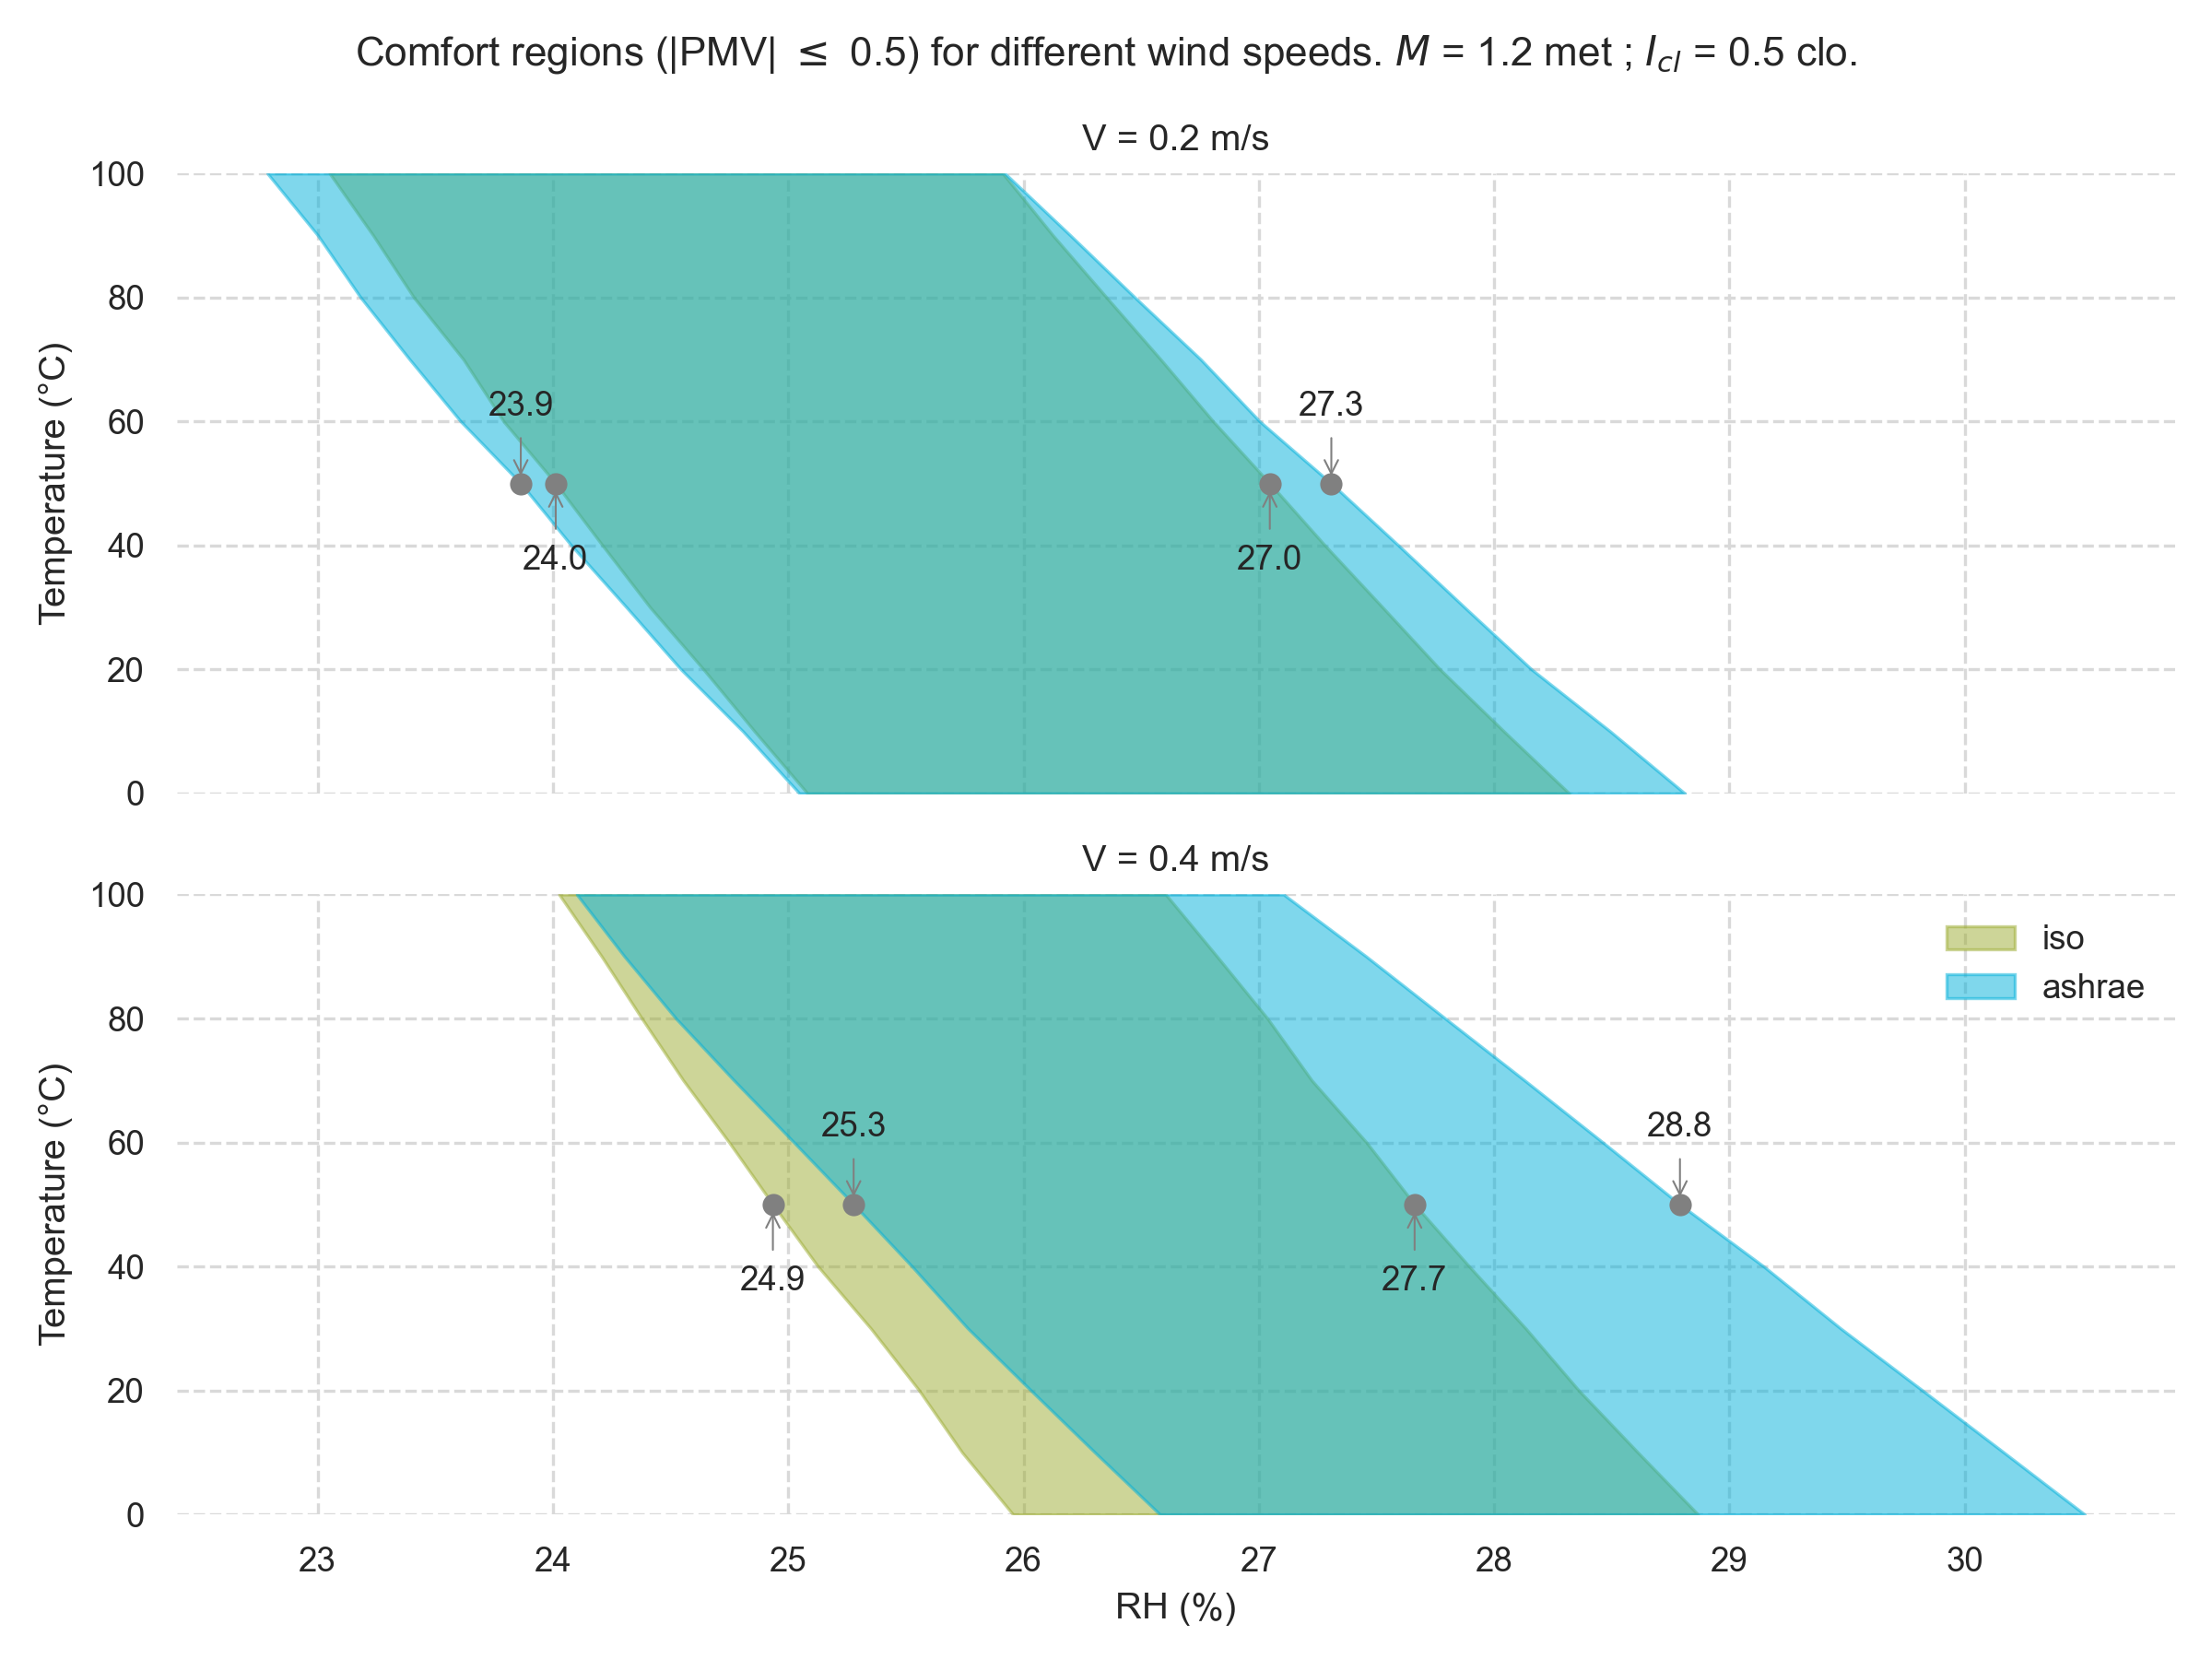
\includegraphics[width=1\textwidth]{figures/pmv_comfort_regions}
    \caption{Comfort regions ($|$\ac{pmv}$|$~$\leq$~\num{0.5}) calculated using \ac{pmv} and \ac{pmv-ce} models for two values of \ac{vr}.
    We set \ac{met}~=~\qty{1.2}{met}, \ac{clor}~=~\qty{0.5}{clo}.
    \label{fig:comfort_regios_pmv_pmvce}}
\end{figure}
The results show that for \ac{vr}~=~\qty{0.4}{\m\per\s} and \ac{rh}~=~\qty{50}{\percent} the comfort regions estimated using the \ac{pmv-ce} is \qty{0.7}{\celsius} wider than the one calculated using the \ac{pmv} and shifted towards warmer temperatures.
For \ac{vr}~=~\qty{0.2}{\m\per\s}, the same difference is \qty{0.4}{\celsius}.

The main rationale for the development of the \ac{pmv-ce} model is that the original \ac{pmv} formulation does not accurately estimate convective and evaporative heat losses from the skin to the environment under elevated air speeds~\cite{huang_applicability_2014}.
The \ac{pmv} does not accurately estimate evaporative heat losses trough sweating because it assumes that sweating is constant and only varies as a function of \ac{met}.
Hence, if sweating is required to maintain the body in thermal equilibrium, the \ac{pmv} model assumes that the body would get hotter.
The human body, on the other hand, uses sweating to maintain a constant body temperature in `warm' environments.
\todo[inline]{true enough, but in the standard the objective is to have a rational physiology model.
The Gagge models are as well or better documented than the Fanger heat balance model, and have been available to Standards users in the ASHRAE Handbook of Fundamentals.}
\todo[inline, color=blue!40]{FT. The PMV CE and the Gagge model are very different, hence, publications about the latter do not justify the implementation proposed in the Std 55}

Despite this claim from the authors of the \ac{pmv-ce}, our analysis has, however, revealed several limitations specific to the \ac{pmv-ce} model, as outlined below.

\begin{enumerate}
    \item Although the \ac{ce} claims to better account for convective heat losses from the skin to the environment due to the air movement, the \ac{pmv-ce} model uses the same underlying equations as the \ac{pmv} model, hence it has the same limitations.
    For example, let's assume that a person is exposed to the following environmental conditions \ac{tdb}~=~\ac{tr}~=~\qty{29}{\celsius}, \ac{rh}~=~\qty{80}{\percent}, \ac{vr}~=~\qty{0.15}{\m\per\s}, they have a \ac{met} of \qty{1}{met} and a \ac{clor} of \qty{0.5}{clo}.
    According to the Gagge's two-node model, which is used to calculate the \ac{set}, this hypothetical person would have \qty{30}{\percent} of their skin covered with sweat.
    Based on the results from \mycite{huang_applicability_2014}, the \ac{pmv} model, in this scenario, cannot accurately predict the \ac{tsv} since the person is sweating.
    However, the only difference between the \ac{pmv} and \ac{pmv-ce} in this scenario, is that the \ac{pmv-ce} accounts for the cooling effect due to the air movement (delta between \qty{0.15}{\m\per\s} and \qty{0.1}{\m\per\s}) which is equal to \qty{.17}{\celsius}.
    Even after reducing both \ac{tdb} and \ac{tr} by the \ac{ce}, the person is still estimated to be sweating.
    Therefore, in this scenario, where the \ac{pmv-ce} should excell compared to the \ac{pmv}, the \ac{pmv-ce} model still fails to accurately predict the \ac{tsv}.
    \todo[inline]{This is really confusing.
    You are evaluating the Cooling Effect in still air, when there is basically no Cooling Effect to evaluate.
    You are using as an example 29C in still air and 80\% RH which of course will cause sweating.
    You are citing skin wettedness values that have not been introduced in this paper (and are not part of any standard). Where did they come from? You allude to results from Huang 2014 that the reader is supposed to know about. The skin wettedness discussion is irrelevant unless you go into a lot more physiological detail here.}
    \item The previous example, highlights another limitation of the \ac{pmv-ce}.
    The assumption of keeping \ac{rh} constant after adjusting \ac{tdb} and \ac{tr} is thermodynamically incorrect since the value of \ac{rh} is dependent on \ac{tdb}.
    The \ac{rh} should be re-calculated, potentially assuming the humidity ratio to be constant, to reflect the new \ac{tdb} value.
    \item It should be noted that over the years, the threshold value of \ac{vr} after which the \ac{ce} is calculated, has been changed from \qty{0.15}{\m\per\s} in the ASHRAE~55:2013~\cite{ASHRAE552013} to \qty{0.2}{\m\per\s} in the ASHRAE~55:2017~\cite{ASHRAE552017, arens_moving_2009} to \qty{0.1}{\m\per\s} in \gls{55}~\cite{ashrae552023}.
    However, these changes were not based on any scientific evidence, despite significantly affecting the output of the model.
    \item The \ac{set} temperature which is used to calculate the \ac{ce}, is defined as the hypothetical isothermal environment at a \ac{rh} of \qty{50}{\percent}, \ac{vr}~$\leq$~\qty{0.1}{\m\per\s}, and \ac{tr}~=~\ac{tdb} in which the total heat loss from the skin of an imaginary occupant wearing clothing, standardized for the activity concerned, is the same as that from a person in the actual environment with actual clothing and activity level~\cite{ashrae552023}.
    However, while \ac{vr}, used to calculate the \ac{pmv-ce}, is set to \qty{0.1}{\m\per\s} the value of \ac{rh} and \ac{clo} are not adjusted to compensate for the fact that \ac{set} fixed the \ac{rh} to \qty{50}{\percent} and standardized the clothing to the activity.
    \todo[inline]{I think this argument is incorrect. SET is only used as a consistent method of obtaining a meaningful delta operative temperature. It does not change the environment. The environment is kept at the original RH.}
    \item Calculating the \ac{pmv-ce} is more computationally intensive and complex since it requires the user to solve two heat balance equations, the \ac{pmv} and the \ac{set} model.
    \todo[inline]{This may or may not be significant. If it is significant, the process could be simplified to a total of three calculations while remaining a rational method. What’s in there now was Tyler’s (CBE’s) choice. Charlie and I have used it in the simpler way. We could propose this to the Standards Committee if we wanted to. We would have to calculate two validation tables for the two approaches.}
\end{enumerate}

\subsection{Other \ac{pmv} Formulations}\label{subsec:other-pmv-formulations}
Several other formulations of the \ac{pmv} model have been proposed.
Among the most notable formulations there are the \ac{pmvs}~\cite{GaggeSET}, \ac{pmvg}~\cite{GaggeSET},  \ac{epmv}~\cite{Toftum2002}, and \ac{athb}~\cite{Schweiker2022}.
\mycite{Yao2022} provides a comprehensive review of different thermal comfort models and compares and describes some of the above-mentioned models.
It should be noted that, while both the \ac{pmvs} and \ac{pmvg} models are based on the \ac{set} model they significantly differ from the \ac{pmv-ce} model.
Both the \ac{pmvs} and \ac{pmvg} are directly calculated within the \ac{set} model using the estimated heat gains and losses from the human body.

Here, we decided to focus on the \ac{pmv} and \ac{pmv-ce} models since they are incorporated in the most widely referenced thermal comfort standards worldwide (\gls{7730} and \gls{55}).

\subsection{Comparison of \ac{pmv} and \ac{pmv-ce}}\label{subsec:comparision-of-pmv-formulations}
To our knowledge, no previous study compared in detail the accuracy of the \ac{pmv} and \ac{pmv-ce} models.
Some notable works that tried to determine the accuracy of the \ac{pmv} model include the work from \mycite{doherty_evaluation_1988} who evaluated the ability of the \ac{pmv} and \ac{set} models to predict several physiological variables (i.e., skin temperature, core temperature, and skin wettedness) under a wide range of still air environments and metabolic rates.
They concluded that the \ac{pmv} model is accurate for simulations of resting subjects, but its accuracy decreases as a function of metabolic rate.
Humphreys and Nicol estimated the effects of measurement and formulation error (i.e., incorrect equations or constants) on predicting thermal sensation using the \ac{pmv}~\cite{Humphreys2000}.
They used the ASHRAE Global Thermal Comfort database~I and determined that the measurement error and the error introduced by the \ac{pmv} model formulation had a similar and non-negligible contribution.
They also determined the validity of the \ac{pmv} for predicting comfort votes collected in field studies~\cite{Humphreys2002}.
They concluded that the \ac{pmv} range of applicability should be significantly reduced and it fails to predict the extent of thermal dissatisfaction of people in buildings.
The \ac{pmv} was free from bias only when it was used to predict thermal neutrality~\cite{Humphreys2002}.
\mycite{Cheung2019} determined the accuracy of the \ac{pmv} model, by comparing its results with the \ac{tsv} from the ASHRAE Global Thermal Comfort Database II.
They found that the thermal sensation predicted by the PMV model, on average, is one full thermal sensation scale unit away from the subject’s responses, confirming the results of~\mycite{Humphreys2002}.
\mycite{Cheung2019} also concluded that the accuracy of \ac{pmv} was only \qty{34}{\percent}, the model has a slightly higher prediction accuracy for sensation close to neutrality, but the accuracy declined towards either end of the thermal sensation scale, and it overestimated both hot and cold sensations.
They also found that the Predicted Percentage of Dissatisfied (PPD) failed to predict the percentage of unacceptable votes if the thermal sensation was predicted using the PMV model and suggested its removal from the thermal comfort standard.
These results were confirmed by the analysis of the Chinese Thermal Comfort database~\cite{du_evaluation_2022}.
\mycite{Yao2022} compared the \ac{pmv} and \ac{pmv-ce} models, however, their aim was primarily to compare these two formulations with other adaptive \ac{pmv} formulations, hence, they do not provide a detailed analysis on the prediction accuracy of the two models.
They focused significantly on how the models perform in different climates and when applied to people from different world regions, and their analysis only reports the mean bias of the different models.
This, as depicted by \mycite{Humphreys2000}, does not provide sufficient insights and information in determining which model is more accurate since it does not explain how the model performs over a wide range of environmental, personal conditions, and \ac{tsv}.
Reporting the classification accuracy of the \ac{pmv} formulations when people are grouped by their \ac{tsv} is particularly important for an unbalanced dataset like the \ac{db2} where most of the participants reported to be `neutral'.
Finally, \mycite{Yao2022} only reported the overall bias for the whole dataset, even though the two formulations mainly differ when the \ac{vr} exceeds \qty{0.1}{\m\per\s}.

\subsection{Objectives}\label{subsec:aim-and-objectives}
Choosing between the \ac{pmv} and \ac{pmv-ce} is a source of confusion for researchers, educators and practitioners worldwide since both models are widely used in building codes, guidelines and certification programs.
For example, the WELL certification allows both compliance with \gls{7730} and \gls{55} standards.
In this paper, we compare the accuracy of the \ac{pmv} and \ac{pmv-ce} models used in the \gls{7730} and \gls{55} standards, respectively.
We used the \ac{tsv} recorded in the \acf{db2}.
We aim to determine which \ac{pmv} model is most accurate and the models' applicability limits.